\documentclass[tikz,border=15pt]{standalone}
\usepackage{tikz}
\usetikzlibrary{shapes.geometric, arrows.meta, positioning, fit, calc, backgrounds, decorations.pathreplacing}

\begin{document}

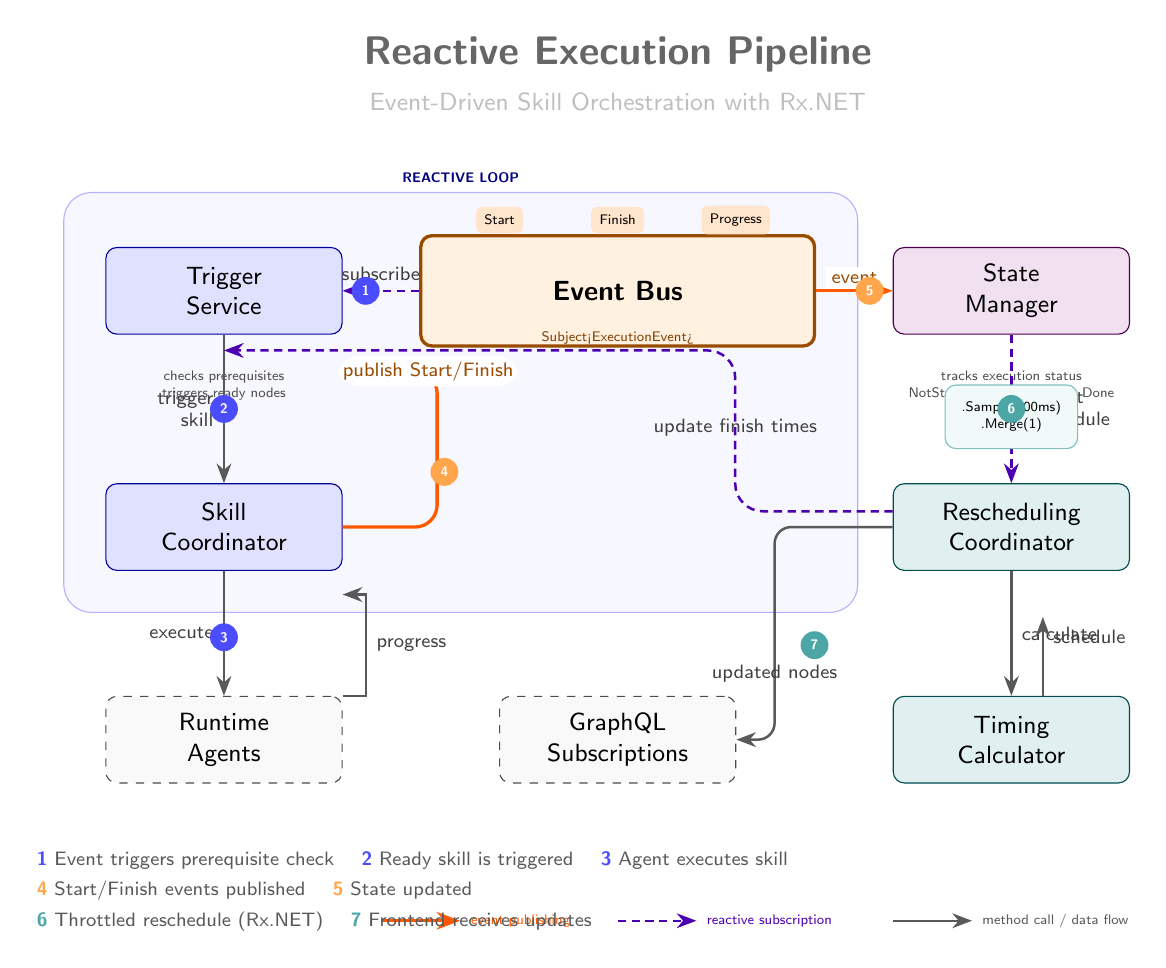
\begin{tikzpicture}[
    % Node styles
    component/.style={
        rectangle,
        rounded corners=4pt,
        draw=#1!60!black,
        fill=#1!12,
        text=black,
        font=\sffamily\small,
        minimum height=1.1cm,
        minimum width=3cm,
        align=center
    },
    eventbus/.style={
        component=orange,
        minimum width=5cm,
        minimum height=1.4cm,
        font=\sffamily\bfseries,
        line width=1.2pt
    },
    trigger/.style={component=blue},
    state/.style={component=violet},
    schedule/.style={component=teal},
    external/.style={component=gray, dashed, fill=gray!5},
    % Arrow styles
    eventarrow/.style={-{Stealth[length=3mm]}, line width=1.2pt, orange!70!red},
    flowarrow/.style={-{Stealth[length=2.5mm]}, line width=0.9pt, gray!70!black},
    reactivearrow/.style={-{Stealth[length=2.5mm]}, line width=0.9pt, blue!60!purple, densely dashed},
    % Label styles
    eventlabel/.style={font=\sffamily\scriptsize, text=orange!60!black, fill=white, inner sep=2pt},
    flowlabel/.style={font=\sffamily\scriptsize, text=gray!50!black},
    note/.style={font=\sffamily\tiny, text=gray!60!black, align=center},
]

% ============================================
% TITLE
% ============================================
\node[font=\sffamily\Large\bfseries, text=gray!80!black] at (0, 6.5) {Reactive Execution Pipeline};
\node[font=\sffamily\small, text=gray!50] at (0, 5.9) {Event-Driven Skill Orchestration with Rx.NET};

% ============================================
% CENTRAL EVENT BUS
% ============================================
\node[eventbus] (eventBus) at (0, 3.5) {Event Bus};
\node[font=\sffamily\tiny, text=orange!50!black] at (0, 2.9) {Subject<ExecutionEvent>};

% Event type badges
\node[fill=orange!20, rounded corners=2pt, font=\sffamily\tiny, inner sep=3pt] at (-1.5, 4.4) {Start};
\node[fill=orange!20, rounded corners=2pt, font=\sffamily\tiny, inner sep=3pt] at (0, 4.4) {Finish};
\node[fill=orange!20, rounded corners=2pt, font=\sffamily\tiny, inner sep=3pt] at (1.5, 4.4) {Progress};

% ============================================
% LEFT SIDE: TRIGGERING & EXECUTION
% ============================================
\node[trigger] (triggerService) at (-5, 3.5) {Trigger\\Service};
\node[trigger] (coordinator) at (-5, 0.5) {Skill\\Coordinator};
\node[external] (agents) at (-5, -2.2) {Runtime\\Agents};

% Trigger service details
\node[note] at (-5, 2.3) {checks prerequisites\\triggers ready nodes};

% ============================================
% RIGHT SIDE: STATE & RESCHEDULING
% ============================================
\node[state] (stateManager) at (5, 3.5) {State\\Manager};
\node[schedule] (rescheduler) at (5, 0.5) {Rescheduling\\Coordinator};
\node[schedule] (scheduler) at (5, -2.2) {Timing\\Calculator};

% State manager details
\node[note] at (5, 2.3) {tracks execution status\\NotStarted → Running → Done};

% ============================================
% BOTTOM: FRONTEND
% ============================================
\node[external] (frontend) at (0, -2.2) {GraphQL\\Subscriptions};

% ============================================
% MAIN REACTIVE FLOWS
% ============================================

% TriggerService subscribes to EventBus
\draw[reactivearrow] (eventBus.west) -- node[above, flowlabel] {subscribe} (triggerService.east);

% TriggerService triggers Coordinator
\draw[flowarrow] (triggerService.south) -- node[left, flowlabel, align=right] {trigger\\skill} (coordinator.north);

% Coordinator calls Agents
\draw[flowarrow] (coordinator.south) -- node[left, flowlabel] {execute} (agents.north);

% Agents return progress to Coordinator
\draw[flowarrow] (agents.north east) -- ++(0.3, 0) |- node[right, flowlabel, pos=0.25] {progress} ([yshift=-0.3cm]coordinator.south east);

% Coordinator publishes events to EventBus
\draw[eventarrow, rounded corners=8pt] (coordinator.east) -- ++(1.2, 0) |- node[eventlabel, pos=0.75] {publish Start/Finish} ([yshift=-0.3cm]eventBus.south west);

% EventBus notifies StateManager
\draw[eventarrow] (eventBus.east) -- node[above, eventlabel] {event} (stateManager.west);

% StateManager triggers rescheduling
\draw[reactivearrow] (stateManager.south) -- node[right, flowlabel, align=left] {request\\reschedule} (rescheduler.north);

% Rescheduler calls Scheduler
\draw[flowarrow] (rescheduler.south) -- node[right, flowlabel] {calculate} (scheduler.north);

% Scheduler returns to Rescheduler
\draw[flowarrow] ([xshift=0.4cm]scheduler.north) -- ++(0, 0.5) -- node[right, flowlabel] {schedule} ++(0, 0.5);

% Rescheduler publishes to Frontend
\draw[flowarrow, rounded corners=6pt] (rescheduler.west) -- ++(-1.5, 0) |- node[flowlabel, pos=0.3, below] {updated nodes} (frontend.east);

% Rescheduler updates TriggerService (adaptive skills)
\draw[reactivearrow, rounded corners=10pt] ([yshift=0.2cm]rescheduler.west) -- ++(-2, 0) |- node[flowlabel, pos=0.2, above] {update finish times} ([yshift=-0.2cm]triggerService.south);

% ============================================
% RX.NET THROTTLE BOX
% ============================================
\node[draw=teal!50, fill=teal!5, rounded corners=4pt, font=\sffamily\tiny, align=center, inner sep=6pt]
    (throttle) at (5, 1.9) {
        .Sample(500ms)\\
        .Merge(1)
    };

% ============================================
% REACTIVE LOOP HIGHLIGHT
% ============================================
\begin{scope}[on background layer]
    \node[draw=blue!30, fill=blue!3, rounded corners=10pt, fit=(triggerService)(coordinator)(eventBus), inner sep=15pt] (loopbox) {};
\end{scope}
\node[font=\sffamily\tiny\bfseries, text=blue!50!black, anchor=south] at (loopbox.north) {REACTIVE LOOP};

% ============================================
% LEGEND
% ============================================
\begin{scope}[shift={(-3, -4.5)}]
    \draw[eventarrow] (0,0) -- (1,0) node[right, font=\sffamily\tiny] {event publishing};
    \draw[reactivearrow] (3,0) -- (4,0) node[right, font=\sffamily\tiny] {reactive subscription};
    \draw[flowarrow] (6.5,0) -- (7.5,0) node[right, font=\sffamily\tiny] {method call / data flow};
\end{scope}

% ============================================
% NUMBERED FLOW ANNOTATIONS
% ============================================
\node[circle, fill=blue!70, text=white, font=\sffamily\tiny\bfseries, inner sep=2pt] at (-3.2, 3.5) {1};
\node[circle, fill=blue!70, text=white, font=\sffamily\tiny\bfseries, inner sep=2pt] at (-5, 2) {2};
\node[circle, fill=blue!70, text=white, font=\sffamily\tiny\bfseries, inner sep=2pt] at (-5, -0.9) {3};
\node[circle, fill=orange!70, text=white, font=\sffamily\tiny\bfseries, inner sep=2pt] at (-2.2, 1.2) {4};
\node[circle, fill=orange!70, text=white, font=\sffamily\tiny\bfseries, inner sep=2pt] at (3.2, 3.5) {5};
\node[circle, fill=teal!70, text=white, font=\sffamily\tiny\bfseries, inner sep=2pt] at (5, 2) {6};
\node[circle, fill=teal!70, text=white, font=\sffamily\tiny\bfseries, inner sep=2pt] at (2.5, -1) {7};

% Flow description
\node[font=\sffamily\scriptsize, text=gray!70!black, align=left, anchor=north west] at (-7.5, -3.5) {
    \textcolor{blue!70}{\textbf{1}} Event triggers prerequisite check \quad
    \textcolor{blue!70}{\textbf{2}} Ready skill is triggered \quad
    \textcolor{blue!70}{\textbf{3}} Agent executes skill\\[3pt]
    \textcolor{orange!70}{\textbf{4}} Start/Finish events published \quad
    \textcolor{orange!70}{\textbf{5}} State updated\\[3pt]
    \textcolor{teal!70}{\textbf{6}} Throttled reschedule (Rx.NET) \quad
    \textcolor{teal!70}{\textbf{7}} Frontend receives updates
};

\end{tikzpicture}

\end{document}
